% ============================================================================
% CHAPTER 10: MARKET ANALYSIS
% ============================================================================

\chapter{Market Analysis}
\label{ch:market}

This chapter provides a comprehensive comparison of our contract-based approach with existing commercial and open-source UAV control systems.

\section{Current UAV Control Landscape}

\subsection{Market Segments}

\begin{figure}[htbp]
    \centering
    \begin{tikzpicture}[
        segment/.style={
            draw,
            rounded corners=5pt,
            minimum width=4cm,
            minimum height=2cm,
            align=center,
            font=\small
        }
    ]
        % Segments
        \node[segment, fill=red!20] (consumer) at (0,4) {
            \textbf{Consumer}\\
            DJI, Parrot\\
            \$500--\$5,000
        };

        \node[segment, fill=orange!20] (prosumer) at (5,4) {
            \textbf{Prosumer}\\
            DJI Enterprise, Autel\\
            \$5,000--\$20,000
        };

        \node[segment, fill=yellow!20] (commercial) at (10,4) {
            \textbf{Commercial}\\
            Skydio, senseFly\\
            \$20,000--\$100,000
        };

        \node[segment, fill=green!20] (enterprise) at (2.5,1) {
            \textbf{Enterprise/Defense}\\
            Boeing, Northrop Grumman\\
            \$100,000+
        };

        \node[segment, fill=blue!20] (research) at (7.5,1) {
            \textbf{Research/Open Source}\\
            PX4, ArduPilot\\
            Cost of hardware
        };

        % Our position
        \node[segment, fill=contractpurple!30, line width=2pt, draw=contractpurple] (ours) at (5,0) {
            \textbf{Contract-Based (Ours)}\\
            Formal verification\\
            Safety-critical applications
        };

        % Arrows showing target markets
        \draw[-{Stealth}, thick, contractpurple] (ours) -- (commercial);
        \draw[-{Stealth}, thick, contractpurple] (ours) -- (enterprise);
    \end{tikzpicture}
    \caption{UAV market segments and positioning}
    \label{fig:market_segments}
\end{figure}

\section{Major Competitors}

\subsection{DJI (Consumer \& Enterprise)}

\textbf{Company Profile:}
\begin{itemize}
    \item World's largest consumer drone manufacturer ($\sim$70\% market share)
    \item Products: Mavic, Phantom, Matrice series
    \item Headquarters: Shenzhen, China
\end{itemize}

\textbf{Control System:}
\begin{itemize}
    \item Proprietary closed-source flight controller
    \item Vision-based obstacle avoidance (APAS)
    \item Geofencing and altitude limits
    \item Return-to-Home (RTH) failsafe
\end{itemize}

\textbf{Limitations:}
\begin{itemize}
    \item No formal safety guarantees
    \item Black-box decision making
    \item Limited customization
    \item Geopolitical concerns for defense applications
\end{itemize}

\subsection{Skydio (AI-Powered Autonomy)}

\textbf{Company Profile:}
\begin{itemize}
    \item US-based, founded by MIT roboticists
    \item Products: Skydio 2, Skydio X2
    \item Focus: Autonomous navigation, inspection
\end{itemize}

\textbf{Control System:}
\begin{itemize}
    \item Deep learning-based visual navigation
    \item 360° obstacle avoidance with 6 cameras
    \item Motion planning with learned models
    \item Dock-based autonomous operations
\end{itemize}

\textbf{Limitations:}
\begin{itemize}
    \item AI decisions not formally verifiable
    \item Requires extensive compute (NVIDIA Tegra)
    \item Training data biases unknown
    \item Certification challenges for safety-critical use
\end{itemize}

\subsection{PX4 (Open Source)}

\textbf{Project Profile:}
\begin{itemize}
    \item Open-source flight control software
    \item Supported by Dronecode Foundation
    \item Used by: Intel, Qualcomm, Auterion
\end{itemize}

\textbf{Control System:}
\begin{itemize}
    \item Cascaded PID controllers
    \item EKF-based state estimation (EKF2)
    \item Mission planning with MAVLink
    \item Geofence and failsafe modes
\end{itemize}

\textbf{Limitations:}
\begin{itemize}
    \item Heuristic safety mechanisms
    \item No formal contracts between modules
    \item Manual tuning required
    \item Limited adaptation to disturbances
\end{itemize}

\subsection{ArduPilot (Open Source)}

\textbf{Project Profile:}
\begin{itemize}
    \item Oldest and most widely used open-source autopilot
    \item Community-driven development
    \item Supports: Copter, Plane, Rover, Sub
\end{itemize}

\textbf{Control System:}
\begin{itemize}
    \item Similar to PX4 (cascaded PID)
    \item Extended Kalman Filter
    \item Lua scripting for customization
    \item Extensive failsafe options
\end{itemize}

\textbf{Limitations:}
\begin{itemize}
    \item Same as PX4 (no formal verification)
    \item Complex codebase, difficult to certify
    \item Reactive-only adaptation
\end{itemize}

\section{Comparative Analysis}

\subsection{Safety Mechanisms}

\begin{table}[htbp]
    \centering
    \caption{Safety mechanism comparison}
    \label{tab:safety_comparison}
    \small
    \begin{tabular}{@{}p{3cm}ccccc@{}}
        \toprule
        \textbf{Feature} & \textbf{DJI} & \textbf{Skydio} & \textbf{PX4} & \textbf{ArduPilot} & \textbf{Ours} \\
        \midrule
        Formal verification & \xmark & \xmark & \xmark & \xmark & \cmark \\
        A/G contracts & \xmark & \xmark & \xmark & \xmark & \cmark \\
        Predictive adaptation & \xmark & Partial & \xmark & \xmark & \cmark \\
        CBF safety layer & \xmark & \xmark & \xmark & \xmark & \cmark \\
        Pre-flight verification & \xmark & \xmark & \xmark & \xmark & \cmark \\
        Geofencing & \cmark & \cmark & \cmark & \cmark & \cmark \\
        Return-to-Home & \cmark & \cmark & \cmark & \cmark & \cmark \\
        Obstacle avoidance & \cmark & \cmark & Partial & Partial & Future \\
        \bottomrule
    \end{tabular}
\end{table}

\subsection{Control Architecture}

\begin{table}[htbp]
    \centering
    \caption{Control architecture comparison}
    \label{tab:control_comparison}
    \small
    \begin{tabular}{@{}p{3cm}ccccc@{}}
        \toprule
        \textbf{Feature} & \textbf{DJI} & \textbf{Skydio} & \textbf{PX4} & \textbf{ArduPilot} & \textbf{Ours} \\
        \midrule
        Primary controller & PID & Learned & PID & PID & PID + H-$\infty$ \\
        Adaptive switching & \xmark & \xmark & \xmark & \xmark & \cmark \\
        Robust control & Unknown & Unknown & Limited & Limited & H-$\infty$ \\
        Disturbance rejection & Reactive & Learned & Reactive & Reactive & Predictive \\
        State estimation & Proprietary & Visual-inertial & EKF2 & EKF & Contract EKF \\
        \bottomrule
    \end{tabular}
\end{table}

\subsection{Certification Readiness}

\begin{table}[htbp]
    \centering
    \caption{Certification readiness comparison}
    \label{tab:cert_comparison}
    \small
    \begin{tabular}{@{}p{4cm}ccccc@{}}
        \toprule
        \textbf{Aspect} & \textbf{DJI} & \textbf{Skydio} & \textbf{PX4} & \textbf{ArduPilot} & \textbf{Ours} \\
        \midrule
        DO-178C potential & Low & Low & Medium & Medium & High \\
        Traceable requirements & \xmark & \xmark & Partial & Partial & \cmark \\
        Formal specifications & \xmark & \xmark & \xmark & \xmark & \cmark \\
        Test coverage & Unknown & Unknown & Partial & Partial & Contract-based \\
        Decision transparency & \xmark & \xmark & \cmark & \cmark & \cmark \\
        \bottomrule
    \end{tabular}
\end{table}

\section{Feature Comparison Matrix}

\begin{table}[htbp]
    \centering
    \caption{Comprehensive feature comparison}
    \label{tab:feature_matrix}
    \footnotesize
    \begin{tabular}{@{}p{4.5cm}p{1.8cm}p{1.8cm}p{1.8cm}p{1.8cm}p{2cm}@{}}
        \toprule
        \textbf{Feature} & \textbf{DJI} & \textbf{Skydio} & \textbf{PX4} & \textbf{ArduPilot} & \textbf{Ours} \\
        \midrule
        \multicolumn{6}{l}{\textit{Safety \& Verification}} \\
        Formal safety guarantees & No & No & No & No & \textbf{Yes} \\
        Contract-based interfaces & No & No & No & No & \textbf{Yes} \\
        Predictive violation detection & No & Partial & No & No & \textbf{Yes} \\
        Runtime safety enforcement & Geofence & Avoidance & Geofence & Geofence & \textbf{CBF} \\
        \midrule
        \multicolumn{6}{l}{\textit{Adaptation}} \\
        Multi-controller support & No & No & Limited & Limited & \textbf{Yes} \\
        Automatic switching & No & No & No & No & \textbf{Yes} \\
        Wind adaptation & Reactive & Learned & Reactive & Reactive & \textbf{Predictive} \\
        GPS-denied operation & Limited & Good & Limited & Limited & \textbf{Supported} \\
        \midrule
        \multicolumn{6}{l}{\textit{Planning}} \\
        Horizon planning & No & Yes & No & No & \textbf{Yes} \\
        Contract composition & No & No & No & No & \textbf{Yes (Pacti)} \\
        Pre-flight verification & Basic & Basic & Basic & Basic & \textbf{Formal} \\
        Mission feasibility & No & Partial & No & No & \textbf{Yes} \\
        \midrule
        \multicolumn{6}{l}{\textit{Transparency}} \\
        Open source & No & No & Yes & Yes & Yes \\
        Decision explainability & Low & Low & High & High & \textbf{Very High} \\
        Audit trail & Limited & Limited & Yes & Yes & \textbf{Contract logs} \\
        \bottomrule
    \end{tabular}
\end{table}

\section{Unique Differentiators}

\subsection{What Sets Us Apart}

\begin{enumerate}
    \item \textbf{Formal Verification:} Only system with mathematically provable safety properties through A/G contracts.

    \item \textbf{Predictive Adaptation:} Horizon planning anticipates problems before they occur, unlike reactive approaches.

    \item \textbf{Principled Controller Switching:} Contract-based switching with formal guarantees, not heuristic thresholds.

    \item \textbf{Defense-in-Depth:} Multiple safety layers (planning, supervision, CBF) with formal interfaces.

    \item \textbf{Certification Path:} Contract-based design directly supports DO-178C compliance.
\end{enumerate}

\subsection{Technology Advantages}

\begin{figure}[htbp]
    \centering
    \begin{tikzpicture}[
        scale=0.9,
        adv/.style={
            draw,
            rounded corners=5pt,
            minimum width=5cm,
            minimum height=1.2cm,
            align=center,
            font=\small,
            fill=contractpurple!20
        }
    ]
        \node[adv] at (0,3) {\textbf{Pacti Library}\\Polyhedral contract composition};
        \node[adv] at (0,1.5) {\textbf{A/G Contracts}\\Formal component interfaces};
        \node[adv] at (0,0) {\textbf{H-$\infty$ Control}\\Robust disturbance rejection};
        \node[adv] at (0,-1.5) {\textbf{CBF Safety}\\Forward invariance guarantees};
        \node[adv] at (0,-3) {\textbf{Horizon Planning}\\Predictive contract cascade};

        % Arrows
        \foreach \y in {3,1.5,0,-1.5} {
            \draw[-{Stealth}, thick, contractpurple] (3,\y) -- (4,\y);
        }

        % Result
        \node[draw, rounded corners=10pt, fill=green!20, minimum width=4cm, minimum height=3cm, align=center]
            at (6.5,0) {\textbf{Provably Safe}\\
            \textbf{Adaptive UAV}\\
            \textbf{Control}};
    \end{tikzpicture}
    \caption{Technology stack providing unique advantages}
    \label{fig:tech_advantages}
\end{figure}

\section{Target Markets}

\subsection{Primary Markets}

\begin{enumerate}
    \item \textbf{Urban Air Mobility (UAM):}
    \begin{itemize}
        \item Passenger-carrying drones require certification
        \item Our formal methods enable compliance path
        \item Market size: \$1.5B by 2030 (projected)
    \end{itemize}

    \item \textbf{Medical Delivery:}
    \begin{itemize}
        \item Blood, organ, medication delivery
        \item Reliability and safety critical
        \item Growing regulatory acceptance
    \end{itemize}

    \item \textbf{Infrastructure Inspection:}
    \begin{itemize}
        \item Power lines, bridges, pipelines
        \item Predictable behavior near structures
        \item Bounded tracking error guarantees
    \end{itemize}

    \item \textbf{Defense \& Government:}
    \begin{itemize}
        \item Formal verification required for autonomy
        \item US-origin technology preferred
        \item Transparent decision-making
    \end{itemize}
\end{enumerate}

\subsection{Market Opportunity}

\begin{figure}[htbp]
    \centering
    \begin{tikzpicture}
        \begin{axis}[
            width=12cm, height=7cm,
            ybar,
            ylabel={Market Size (\$B)},
            xlabel={Year},
            xtick=data,
            symbolic x coords={2024, 2025, 2026, 2027, 2028, 2029, 2030},
            ymin=0, ymax=60,
            bar width=15pt,
            legend pos=north west,
            grid=major
        ]
            % Total UAV market
            \addplot[fill=gray!50] coordinates {
                (2024, 25) (2025, 29) (2026, 34) (2027, 39)
                (2028, 45) (2029, 51) (2030, 58)
            };

            % Safety-critical segment
            \addplot[fill=contractpurple!50] coordinates {
                (2024, 3) (2025, 4) (2026, 5.5) (2027, 7.5)
                (2028, 10) (2029, 13) (2030, 17)
            };

            \legend{Total UAV Market, Safety-Critical Segment}
        \end{axis}
    \end{tikzpicture}
    \caption{Projected UAV market growth with safety-critical segment}
    \label{fig:market_growth}
\end{figure}

\section{Competitive Strategy}

\subsection{Positioning}

Position as the \textbf{``safety verification layer''} for UAV systems:
\begin{itemize}
    \item Complement existing platforms (PX4, ArduPilot)
    \item Provide formal verification capabilities
    \item Enable certification for safety-critical applications
    \item License technology to OEMs
\end{itemize}

\subsection{Go-to-Market}

\begin{enumerate}
    \item \textbf{Phase 1:} Research partnerships with aerospace companies
    \item \textbf{Phase 2:} Integration with open-source platforms
    \item \textbf{Phase 3:} Certification pilot programs
    \item \textbf{Phase 4:} Commercial licensing
\end{enumerate}

\section{Regulatory Landscape}

\begin{table}[htbp]
    \centering
    \caption{Relevant regulatory standards}
    \label{tab:regulations}
    \begin{tabular}{@{}p{3cm}p{9cm}@{}}
        \toprule
        \textbf{Standard} & \textbf{Relevance} \\
        \midrule
        DO-178C & Software certification for airborne systems; our contract-based approach supports compliance \\
        DO-254 & Hardware certification; not directly applicable but complementary \\
        ASTM F3269 & Standard for UAV command and control; formal interfaces align well \\
        JARUS SORA & Specific Operations Risk Assessment; contracts can document safety mitigations \\
        14 CFR Part 107 & FAA small UAS rules; waiver applications benefit from formal guarantees \\
        \bottomrule
    \end{tabular}
\end{table}

\section{SWOT Analysis}

\begin{figure}[htbp]
    \centering
    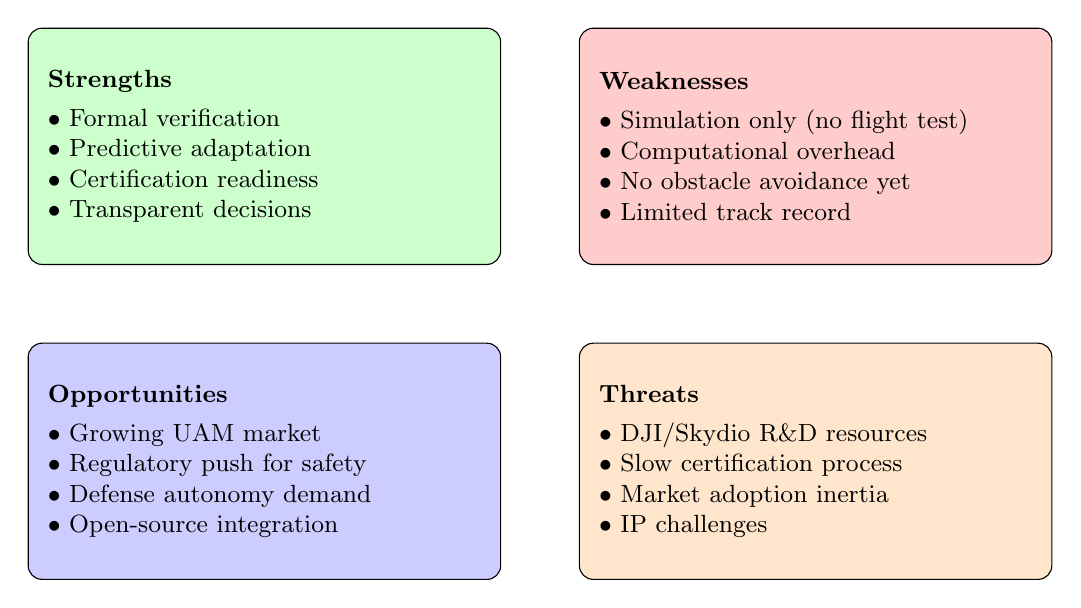
\begin{tikzpicture}[
        box/.style={
            draw,
            rounded corners=5pt,
            minimum width=6cm,
            minimum height=3cm,
            align=left,
            font=\small,
            text width=5.5cm
        }
    ]
        % Strengths
        \node[box, fill=green!20] (s) at (0,2.5) {
            \textbf{Strengths}\\[3pt]
            $\bullet$ Formal verification\\
            $\bullet$ Predictive adaptation\\
            $\bullet$ Certification readiness\\
            $\bullet$ Transparent decisions
        };

        % Weaknesses
        \node[box, fill=red!20] (w) at (7,2.5) {
            \textbf{Weaknesses}\\[3pt]
            $\bullet$ Simulation only (no flight test)\\
            $\bullet$ Computational overhead\\
            $\bullet$ No obstacle avoidance yet\\
            $\bullet$ Limited track record
        };

        % Opportunities
        \node[box, fill=blue!20] (o) at (0,-1.5) {
            \textbf{Opportunities}\\[3pt]
            $\bullet$ Growing UAM market\\
            $\bullet$ Regulatory push for safety\\
            $\bullet$ Defense autonomy demand\\
            $\bullet$ Open-source integration
        };

        % Threats
        \node[box, fill=orange!20] (t) at (7,-1.5) {
            \textbf{Threats}\\[3pt]
            $\bullet$ DJI/Skydio R\&D resources\\
            $\bullet$ Slow certification process\\
            $\bullet$ Market adoption inertia\\
            $\bullet$ IP challenges
        };
    \end{tikzpicture}
    \caption{SWOT analysis of contract-based approach}
    \label{fig:swot}
\end{figure}

\section{Conclusion}

The contract-based approach offers unique value in the growing safety-critical UAV market:

\begin{itemize}
    \item \textbf{No direct competitor} offers formal A/G contracts with predictive horizon planning
    \item \textbf{Clear certification path} compared to AI-based or heuristic approaches
    \item \textbf{Growing market demand} for verifiable autonomous systems
    \item \textbf{Technical differentiation} through Pacti, H-$\infty$, and CBF integration
\end{itemize}

The primary barrier is demonstrating flight-test validation, which would significantly strengthen market position.

